\documentclass{article}
\usepackage[utf8]{inputenc}
\usepackage[margin=3.0cm]{geometry}
\usepackage{minted}
\usepackage{amssymb}
\usepackage{amsthm}
\usepackage{amsmath}
\usepackage{graphicx}
\usepackage{bbm}
\usepackage{subcaption}
\pagestyle{empty}
\usepackage[table]{xcolor}
\newcommand{\wo}{\mathbbm{w}}

\pdfinfo{
/Title (report2)
/Author (Felipe Salvatore)}
\setcounter{secnumdepth}{0}  


\title{Report: assigment 2}
\author{Felipe Salvatore\\
\texttt{felipessalvador@googlemail.com}}
\begin{document}
\maketitle
\section{1}
\textbf{1a)} 
\begin{minted}{python}
def softmax(x):
    # ## YOUR CODE HERE
    all_constants = - tf.reduce_max(x, axis=1)
    x = x + tf.expand_dims(all_constants, 1)
    x = tf.exp(x)
    all_sums = tf.reduce_sum(x, 1)
    all_sums = tf.pow(all_sums, -1)
    out = x*tf.expand_dims(all_sums, 1)
    # ## END YOUR CODE
    return out
\end{minted}


\textbf{1b)}
\begin{minted}{python}
def cross_entropy_loss(y, yhat):
    # ## YOUR CODE HERE
    y = tf.cast(y, tf.float32)
    yhat = tf.log(yhat)
    out = - tf.reduce_sum(y*yhat)
    out = tf.reshape(out, (1,))
    # ## END YOUR CODE
    return out
\end{minted}

\textbf{1c)} The placeholders variables are like their name suggest a placeholder for a tensor. We use it to form a computational graph before the training. In the training stage we use the dictionary feed\_dict to 'load' the placeholders variables with real tensors.

\begin{minted}{python}
    def add_placeholders(self):
        # ## YOUR CODE HERE
        self.input_placeholder = tf.placeholder(tf.float32,
                                                shape=[self.config.batch_size,
                                                       self.config.n_features],
                                                name="input_placeholder")
        self.labels_placeholder = tf.placeholder(tf.int32,
                                                 shape=[self.config.batch_size,
                                                        self.config.n_classes],
                                                 name="labels_placeholder")
        # ## END YOUR CODE

    def create_feed_dict(self, input_batch, label_batch):
        # ## YOUR CODE HERE
        feed_dict = {self.input_placeholder: input_batch,
                     self.labels_placeholder: label_batch}
        # ## END YOUR CODE
        return feed_dict
\end{minted}

\textbf{1d)}
\begin{minted}{python}
    def add_model(self, input_data):
        Wshape = [self.config.n_features, self.config.n_classes]
        bshape = [self.config.batch_size, self.config.n_classes]
        Winit = tf.zeros(Wshape)
        binit = tf.zeros(bshape)

        with tf.variable_scope("linear-model"):
            W = tf.get_variable("weights", dtype='float32', initializer=Winit)
            b = tf.get_variable("bias", dtype='float32', initializer=binit)
            out = softmax(tf.matmul(input_data, W) + b)
        # ## END YOUR CODE
        return out

    def add_loss_op(self, pred):
        # ## YOUR CODE HERE
        loss = cross_entropy_loss(self.labels_placeholder,
                                  pred)
        # ## END YOUR CODE
        return loss
\end{minted}


\textbf{1e)}
\begin{minted}{python}
    def add_training_op(self, loss):
        # ## YOUR CODE HERE
        optimizer = tf.train.GradientDescentOptimizer(self.config.lr)
        train_op = optimizer.minimize(loss)

        # ## END YOUR CODE
        return train_op
\end{minted}
All the basic operations in TensorFlow have attached
gradient operations. And so with the use of backpropagation TensorFlow computes the gradients for all variables in the computation graph.

\section{2}
We shall first understand \textbf{the Named Entity Recognition (NER) window model}. Suppose we have a corpus with a vocabulary $V =[\wo_{1}, \dots, \wo_{|V|}]$ (we are assuming that every word $\wo$ correspond to an index $i \in \{1, \dots, |V|\}$), a number $C$ of name entity categories (null-class,Person, Location, etc.) and a matrix $L \in \mathbb{R}^{|V|,d}$ where each row $i$ correspond to the word embedding of size $d$ of the word $\wo_{i}$. Now we can choose the parameters $m$ and $H$ to be the size window and the size of the hidden layer, respectively. Let $n = (2m+1)d$, $W \in \mathbb{R}^{n,H}$, $b_{1} \in \mathbb{R}^{H}$, $U \in \mathbb{R}^{H,C}$ and $b^{2} \in \mathbb{R}^{C}$. We assume that the training dataset is compose by training samples of the form $([\wo_{t-m}, \dots, \wo_{t}, \dots, \wo_{t+m}],c)$ where $c \in \{1, \dots, C\}$ ($1$ represent the null-class) -- this sample tell us that the word $ \wo_{t}$ is a name entity of type $c$. Let $y$ be the one-vector representation of $c$ (i.e., $y \in \mathbb{R}^{C}$ such that $y_{i} =1$ iff $i=c$), and let $x_{t-m}, \dots, x_{t}, \dots, x_{t+m}\in \mathbb{R}^{|V|}$ be the one-vector representation of $\wo_{t-m}, \dots, \wo_{t}, \dots, \wo_{t+m}$, respectively. The model is composed by the following equations:
\begin{equation}\label{eq:1}
x^{(t)} = concat([x_{t-m}L, \dots, x_{t}L, \dots, x_{t+m}L])
\end{equation}
 \begin{equation}\label{eq:2}
h = tanh(x^{(t)}W + b_{1})
\end{equation}
\begin{equation}\label{eq:3}
\hat{y} = softmax(hU + b_{2})
\end{equation}
\begin{equation}\label{eq:4}
J(W,b_{1},U,b_{2}) = CE(y,\hat{y}) = -\sum_{s=1}^{C} y_s  \log(\hat{y}_s)
\end{equation}

where $concat$ is the operation of concatenate function and $tanh$ is the hyperbolic tangent function ,i.e.,  $tanh(z) = \frac{e^{z} - e^{-z}}{e^{z} + e^{-z}}$ (we can define this function using the sigmoid function, $tanh(z) = 2sigmoid(2z)-1$). Figure \ref{ner} helps us to visualize the model.

For our particular implementation, let $C=5$ $d=50$, $m=1$, $H=100$ (hence $n=150$) and let $J(\theta)$ be an abbreviation of $J(W,b_{1},U,b_{2})$. Thus, for every training sample the loss function is
\begin{equation}\label{eq:5}
J(\theta) = CE(y,\hat{y}) = -\sum_{s=1}^{5} y_s  \log(\hat{y}_s)
\end{equation}


\begin{figure}
\begin{center}
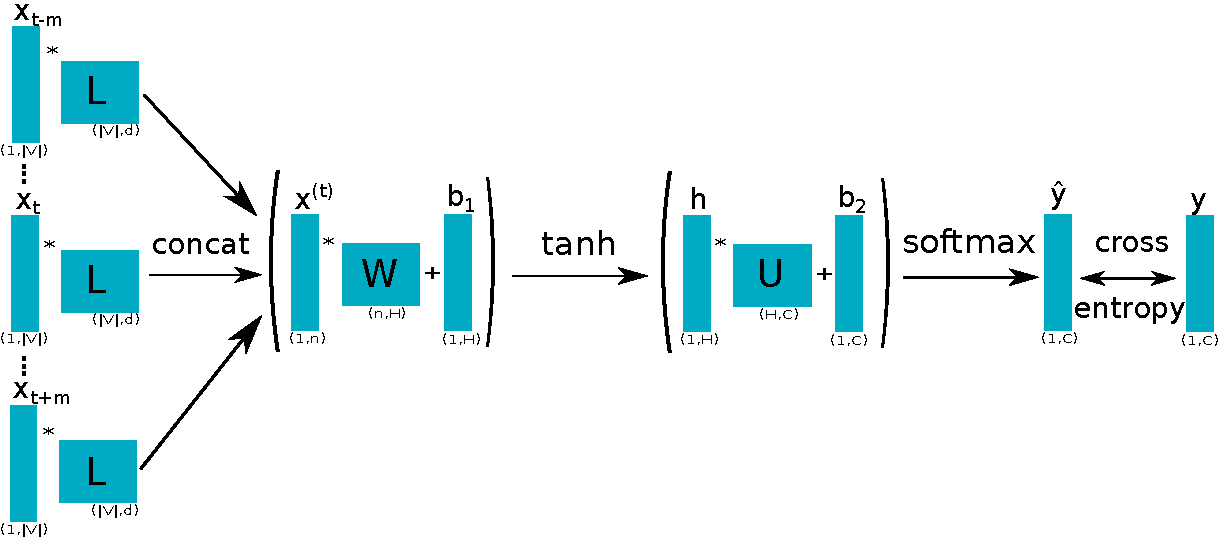
\includegraphics[scale=0.85]{ner.pdf}
\end{center}
\caption{NER window model}
\label{ner}
\end{figure}
\textbf{2a)} Since $tanh(z) = 2\sigma(2z) -1 $ we have that, 
\begin{align*}
tanh^{\prime}(z) & = 2\sigma^{\prime}(2z)2 \\
& =4\sigma^{\prime}(2z) \\
& = 4(\sigma(2z)(1 - \sigma(2z))) \\
& = 4\sigma(2z)(4 - 4\sigma(2z))\\
& =  2(tanh(z)+1)(4 - 2(tanh(z)+1))\\
& = 2((tanh(z)+1)(2 - (tanh(z)+1)))\; .
\end{align*}
Let $\sigma^{(3)} = \hat{y} - y \in \mathbb{R}^{5}$ be the outermost error vector, hence

\begin{equation}\label{eq:6}
\frac{\partial J}{\partial  U} = {h \delta^{(3)}}^{T}
\end{equation}

\begin{equation}\label{eq:7}
\frac{\partial J}{\partial  b_{2}} =  \delta^{(3)}
\end{equation}

\begin{equation}\label{eq:8}
\delta^{(2)} = (\delta^{(3)} {(U)}^{T}) \circ {tanh^{\prime}} (h)
\end{equation}

\begin{equation}\label{eq:9}
\frac{\partial J}{\partial  W} = {x^{(t)} \delta^{(2)}}^{T}
\end{equation}

\begin{equation}\label{eq:10}
\frac{\partial J}{\partial  b_{1}} =  \delta^{(2)}
\end{equation}

First let us define $\frac{\partial J}{\partial  L_{i}}$ for the general case. Using the fact that $\frac{\partial J}{\partial  x^{(t)}}= \delta^{(2)} {(W)}^{T}$ we will define the auxiliary vectors  $v_{1}, \dots, v_{2m+1} \in \mathbb{R}^{d}$ such that for $j \in \{ 1, \dots, 2m+1\}$ 
\begin{equation}\label{eq:11}
v_{j} =  \frac{\partial J}{\partial  x^{(t)}}[(j-1)d +1: jd]
\end{equation}

Let $e$ be the enumeration function of the list $[t-m, \dots, t, \dots, t+m]$, so for $i \in \{ t-m, \dots, t, \dots, t+m \}$

\begin{equation}\label{eq:12}
\frac{\partial J}{\partial  L_{i}} =  v_{e(i)}
\end{equation}

And for $i \notin \{ t-m, \dots, t, \dots, t+m \}$ $\frac{\partial J}{\partial  L_{i}} =0$. Now for the specific case where $m=1$, 

\begin{equation}\label{eq:13}
\frac{\partial J}{\partial  L_{t-1}} =  \frac{\partial J}{\partial  x^{(t)}}[1: d]
\end{equation}
\begin{equation}\label{eq:14}
\frac{\partial J}{\partial  L_{t}} =  \frac{\partial J}{\partial  x^{(t)}}[d+1: 2d]
\end{equation}
\begin{equation}\label{eq:15}
\frac{\partial J}{\partial  L_{t+1}} =  \frac{\partial J}{\partial  x^{(t)}}[2d+1: 3d]
\end{equation}

And for $i \notin \{ t-m, \dots, t, \dots, t+m \}$ $\frac{\partial J}{\partial  L_{i}} =0$.

\textbf{2b)} To add L2 regularization to our model, we can add the following function:
\begin{equation}\label{eq:16}
J_{reg}(\theta) = \frac{\lambda}{2}[\sum_{i=1}^{n}\sum_{j=1}^{H}(W_{i,j})^{2}) + \sum_{i^{\prime}=1}^{H}\sum_{j^{\prime}=1}^{C}(U_{i^{\prime},j^{\prime}})^{2})]
\end{equation}

where $\lambda \in \mathbb{R}$ is the regularization parameter. Hence,

\begin{equation}\label{eq:17}
J_{full}(\theta) =J(\theta) + J_{reg}(\theta)
\end{equation}

The only grandients that change are in respect to $U$ and $W$. Let $\delta^{(3)}$ and $\delta^{(2)}$ be as before; then,

\begin{equation}\label{eq:18}
\frac{\partial J_{full}}{\partial  U} = {h \delta^{(3)}}^{T} + \lambda U 
\end{equation}

\begin{equation}\label{eq:19}
\frac{\partial J_{full}}{\partial  b_{2}} =  \frac{\partial J}{\partial  b_{2}}
\end{equation}

\begin{equation}\label{eq:21}
\frac{\partial J_{full}}{\partial  W} = {x^{(t)} \delta^{(2)}}^{T} + \lambda W 
\end{equation}

\begin{equation}\label{eq:22}
\frac{\partial J_{full}}{\partial  b_{1}} =  \frac{\partial J}{\partial  b_{1}} 
\end{equation}
And for $i \in \{1, \dots, |V|\}$
\begin{equation}\label{eq:23}
\frac{\partial J_{full}}{\partial  L_{i}} =  \frac{\partial J}{\partial  L_{i}} 
\end{equation}

\textbf{2c)}
\begin{minted}{python}
def xavier_weight_init():
    
    def _xavier_initializer(shape, **kwargs):
        
        # ## YOUR CODE HERE
        epsilon = np.sqrt(6.)/np.sqrt(np.sum(shape))
        out = tf.random_uniform(shape,
                                minval=-epsilon,
                                maxval=epsilon,
                                dtype=tf.float32,
                                name='weights')
        # ## END YOUR CODE
        return out
    return _xavier_initializer

\end{minted}

\textbf{2d)}

\begin{minted}{python}
  def add_placeholders(self):
        # ## YOUR CODE HERE
        self.input_placeholder = tf.placeholder(tf.int32,
                                                shape=[None,
                                                       self.config.window_size],
                                                name="input_placeholder")
        self.labels_placeholder = tf.placeholder(tf.float32,
                                                 shape=[None,
                                                        self.config.label_size],
                                                 name="labels_placeholder")
        self.dropout_placeholder = tf.placeholder(tf.float32,
                                                  shape=[],
                                                  name="dropout_value")
        # ## END YOUR CODE

    def create_feed_dict(self, input_batch, dropout, label_batch=None):
        
        # ## YOUR CODE HERE
        if label_batch is None:
            feed_dict = {self.input_placeholder: input_batch,
                         self.dropout_placeholder: dropout}
        else:
            feed_dict = {self.input_placeholder: input_batch,
                         self.labels_placeholder: label_batch,
                         self.dropout_placeholder: dropout}
        # ## END YOUR CODE
        return feed_dict

    def add_embedding(self):
        with tf.device('/cpu:0'):
            # ## YOUR CODE HERE
            Linit = tf.constant_initializer(self.wv)
            L = tf.get_variable("L",
                                shape=[len(self.wv), self.config.embed_size],
                                dtype='float32',
                                initializer=Linit)
            window = tf.nn.embedding_lookup(L, self.input_placeholder)
            window = tf.reshape(window,
                                (-1,
                                 self.config.window_size*self.config.embed_size))
        # ## END YOUR CODE
        return window

  def add_model(self, window):
     
        # ## YOUR CODE HERE
        # shapes
        Wshape = (self.config.window_size*self.config.embed_size,
                  self.config.hidden_size)
        b1shape = (1, self.config.hidden_size)
        Ushape = (self.config.hidden_size, self.config.label_size)
        b2shape = (1, self.config.label_size)

        # initializers
        xavier_initializer = xavier_weight_init()
        Winit = xavier_initializer(Wshape)
        b1init = xavier_initializer(b1shape)
        Uinit = xavier_initializer(Ushape)
        b2init = xavier_initializer(b2shape)

        with tf.variable_scope("Layer"):
            self.W = tf.get_variable("weights",
                                     dtype='float32',
                                     initializer=Winit)
            self.b1 = tf.get_variable("bias",
                                      dtype='float32',
                                      initializer=b1init)
            linear_op = tf.matmul(window, self.W) + self.b1
            first_output = tf.nn.dropout(tf.tanh(linear_op),
                                         self.config.dropout,
                                         name="output")
            tf.add_to_collection("reg", tf.reduce_sum(tf.pow(self.W, 2)))
        with tf.variable_scope("Softmax"):
            self.U = tf.get_variable("weights",
                                     dtype='float32',
                                     initializer=Uinit)
            self.b2 = tf.get_variable("bias",
                                      dtype='float32',
                                      initializer=b2init)
            output = tf.nn.dropout(tf.matmul(first_output, self.U) + self.b2,
                                   self.config.dropout,
                                   name="output")
            tf.add_to_collection("reg", tf.reduce_sum(tf.pow(self.U, 2)))
        # END YOUR CODE
        return output
        
  def add_loss_op(self, y):
            # ## YOUR CODE HERE
        pred = self.labels_placeholder
        cross_entropy = tf.reduce_mean(tf.nn.softmax_cross_entropy_with_logits(y, pred))
        regularization = self.config.l2*0.5*sum(tf.get_collection("reg"))
        loss = cross_entropy + regularization
        # ## END YOUR CODE
        return loss
        
  def add_training_op(self, loss):
     
        # ## YOUR CODE HERE
        optimizer = tf.train.AdamOptimizer(self.config.lr)
        train_op = optimizer.minimize(loss)
        # ## END YOUR CODE
        return train_op
\end{minted}

After some experiments(some related plots can be seen in Figure \ref{NER_e}) we choose the following hyper parameters: $ batch\_size=84, dropout=0.991323729933, lr=0.00365884577219, l2=1.7095245617e-05$. This choice yields val\_loss = $0.156871527433$.

\begin{figure}[H] 
  \begin{subfigure}[b]{0.5\linewidth}
    \centering
    \includegraphics[width=1.05\linewidth]{NER_batch_loss.png} 
    \caption{Validation loss vs batch size} 
    \label{ner_batch} 
    \vspace{4ex}
  \end{subfigure}%% 
  \begin{subfigure}[b]{0.5\linewidth}
    \centering
    \includegraphics[width=1.05\linewidth]{NER_dropout.png} 
    \caption{Validation loss vs dropout} 
    \label{ner_dropout} 
    \vspace{4ex}
  \end{subfigure} 
  \begin{subfigure}[b]{0.5\linewidth}
    \centering
    \includegraphics[width=1.05\linewidth]{NER_lr.png} 
    \caption{validation loss vs learning rate} 
    \label{ner_lr} 
  \end{subfigure}%%
  \begin{subfigure}[b]{0.5\linewidth}
    \centering
    \includegraphics[width=1.05\linewidth]{NER_reg.png} 
    \caption{validation loss vs regularization} 
    \label{ner_reg} 
  \end{subfigure} 
  \caption{Experiments with the NER window model}
  \label{NER_e} 
\end{figure}

\section{3} We will use a \textbf{recurrent neural network (RNN)} to build a language model. Given words $x_{1}, \dots ,x_{n-1}$ a language model predicts the following word $x_{n}$ by modeling:
\[
P(x_{n} = v_{j} | x_{1}, \dots ,x_{n-1})
\]

where $v_{j}$ is a word in the vocabulary. The model can be described as $n-1$ feed-forward neural networks, say $NN^{(1)}, \dots,NN^{(n-1)} $ such that each $NN^{(t)}$ uses an vector from $NN^{(t-1)}$ to perform the computation on its hidden layer. Since the model is the same, we can describe each $NN^{(t)}$ as a time step. Figure \ref{RNN_re} introduces the main idea:     

\begin{figure}[H] 
\begin{center}
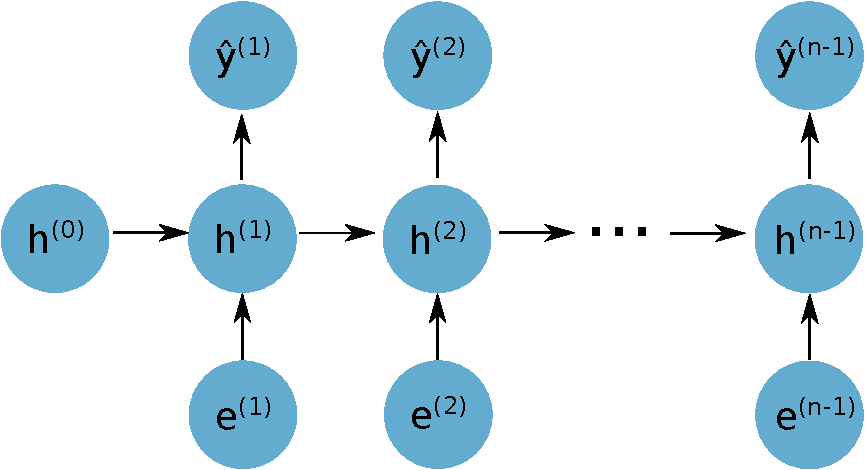
\includegraphics[scale=0.85]{RNN_ball.pdf}
\end{center}
\caption{RNN representation}
\label{RNN_re}
\end{figure}

Since $h^{(n-1)}$ is a function of $h^{(0)},h^{(1)}, \dots, h^{(n-2)}$ we can interpret that at the time step $n-1$ the model $NN^{(n-1)}$ has the "history" of the words $x^{(1)}, x^{(2)}, \dots, x^{(n-2)}$.  


\end{document}
